Robotic assembly is a longstanding challenge, and the NIST Assembly Task Boards are a persistent benchmark~\cite{kimble2020benchmarking}; to the best of our knowledge, no learning-based approaches have solved all tasks on any of the boards. Assembly Task Board \#1 (ATB1) consists of 20 \textit{assembly pair} tasks (a part and its fixed mating geometry on the board) that are relevant for manufacturing, including peg insertion, gear meshing, electrical connector insertion, and nut threading.
Solving this task board is exceptionally challenging for three key reasons:
\textbf{(1)} The sequence for solving the tasks might be unspecified, and not all sequences may be efficient or valid (e.g., solving task N may obstruct the robot from accessing the parts in task N + 1).
\textbf{(2)} Each task is long-horizon, encompassing grasping, transport, and
contact-rich assembly~\cite{narang2022factory}.
Parts may begin in a wide range of poses and require multiple
reorientations before grasping.
During transport, parts may need further reorientation in-hand or
through extrinsic contact.
During assembly, parts may slip, become misaligned, or
jam during insertion or threading~\cite{narang2022factory}, requiring
robust recovery and reexecution.
\textbf{(3)} Solving the tasks requires precise control during complex contact interactions. The parts themselves are small (as small as 4\,mm in diameter), have high geometric detail (e.g., helical threads), and have tight clearances between mating surfaces (as low as zero).
Tasks such as nut threading involve learning helical motion during frictional contact between multiple mating surfaces, during which a nut can tilt, cross-thread, or jam instead of advancing along the bolt~\cite{narang2022factory}.

Learning-free approaches typically rely on planning and strong human priors:
assembly sequence planning~\cite{lozano1993assembly}; customized fixtures,
adapters, and tooling~\cite{kimble2020benchmarking,lian2021benchmarking}; engineered
motion and force primitives~\cite{morgan2023contact}; and tuned admittance,
impedance, or force-motion controllers~\cite{lian2021benchmarking,morgan2023contact}.

Learning-based approaches, on the other hand, can relax some of these constraints, but have shown progress only within a limited scope.
Most efforts have assumed a fixed assembly sequence, heavily constrained the initial poses of parts (e.g., beginning in an already-grasped state)~\cite{luo2021robust}, assumed access to accurate pose estimates, learned specialist rather than multi-task policies~\cite{narang2022factory}, addressed only a subset of tasks on the board~\cite{luo2021robust}, and/or achieved only low-to-moderate success rates by industrial standards.
Success-Guided Sampling (SGS)~\cite{zhang2026balanceddiet}, for example, solves tasks one at a time, but requires a separate policy per task and is considerably less compute-efficient.

We draw inspiration from the landmark AlphaGo series in reinforcement
learning, which surpassed the strongest human Go players.
The progression from AlphaGo to AlphaGo Zero 
showed that learning from a terminal task objective
could encourage superhuman decision-making over long horizons without human demonstrations~\cite{silver2016alphago,silver2017alphagozero}.
In this paper,  we ask whether a similar approach is possible for robotics: can sparse binary task rewards, combined with appropriate training strategies, enable a robot to solve sequences of long-horizon, contact-rich manipulation tasks, perhaps leveraging dexterous behaviors that no human could feasibly specify or demonstrate?
To make learning from sparse task rewards more tractable, we take a seemingly
counterintuitive step: train jointly across heterogeneous assembly pairs differing in geometries, tolerances, and assembly requirements (a nut and its bolt, a gear and its gearshaft, a peg and its hole) from a broad coverage of
initial states, \textbf{converting MDP diversity into a resource rather than a burden}.

\begin{figure}[t]
    \centering
    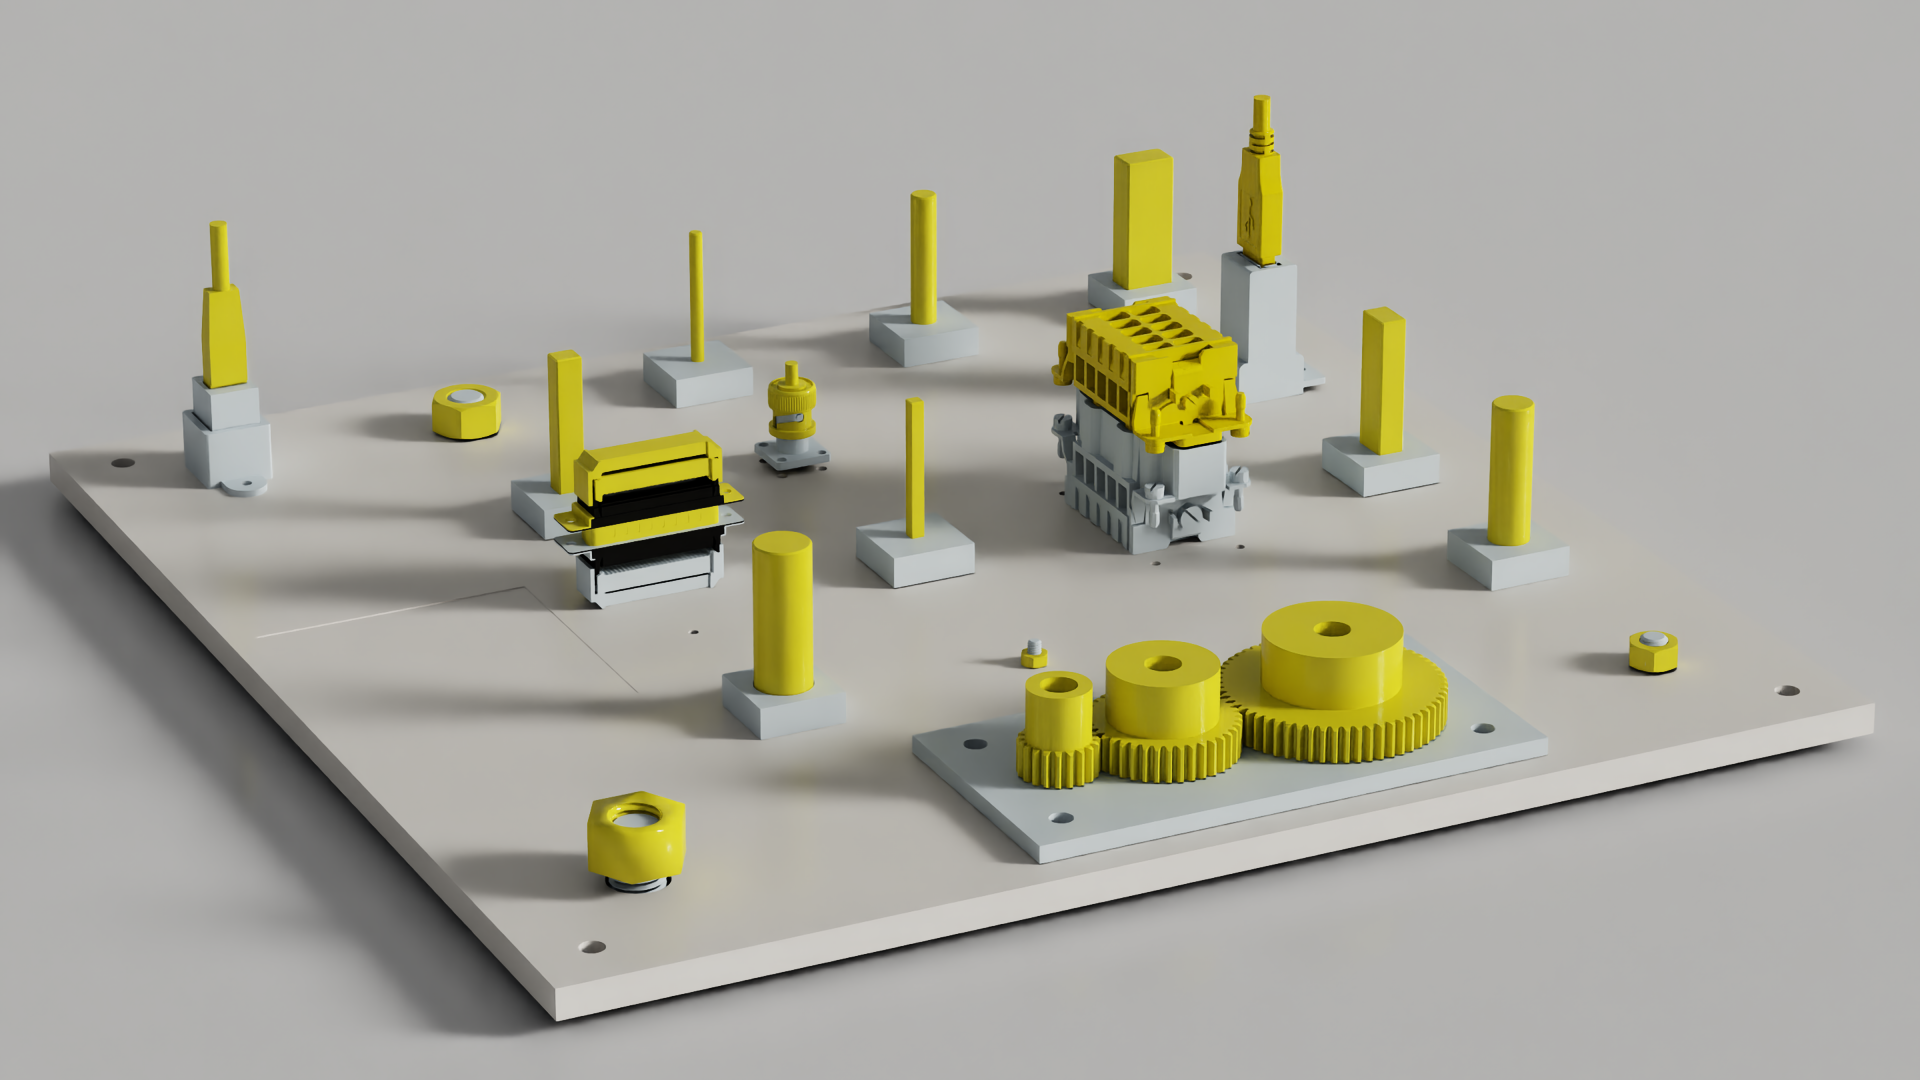
\includegraphics[width=\columnwidth]{figures/overview/nistboard_fully_assembled.png}
    \caption{\textbf{The complete NIST Assembly Task Board \#1 in simulation.}
    Yellow indicates the 20 movable parts in their fully-assembled
    states.}
    \label{fig:nistboard-overview}
\end{figure}

Guided by this insight, we develop AlphaNIST, a learning framework that
trains a \textit{single policy} under sparse binary task rewards across all 20 tasks
on the NIST Assembly Task Board 1 (Fig. \ref{fig:nistboard-overview}).
The policy handles an exceptional range of initial part poses, learns
from point-cloud inputs without first training specialist policies,
and achieves a 98.2\% overall success rate.
Furthermore, the same framework can train policies to complete 10 assembly pairs in
sequence, with a task reward issued only when all pairs are assembled with
\textit{no prescribed order}.
In other words, the policy exhibits planning-like behavior.

Our contributions are the following:
\begin{enumerate}
    \item \textbf{A highly-effective multi-task RL framework} consisting of a novel combination of the following components: A) generation of a cache of assembly-relevant reset states~\cite{yin2026omnireset} over heterogeneous assembly pairs, B) success-guided sampling within the cache~\cite{zhang2026balanceddiet}, C) a unified sparse binary task reward, D) multi-GPU training at scale. These components are supported by careful ablations. All tasks share one training configuration, without per-task tuning or demonstrations.
    \item \textbf{The first multi-task RL policy capable of solving all 20 tasks on the NIST Assembly Task Board 1}. The policy takes point clouds as input; initial part poses are sampled from a wide range, including adverse conditions (e.g., upside-down); and each task can be solved with near-perfect success rates. Positive transfer is observed, where multi-task policies can solve the 20 tasks with higher success rate than individual specialists, including three tasks that the specialists struggle to solve.
    \item \textbf{The first assembly policy capable of solving up to 10 diverse assembly pairs in sequence}, without an explicit hierarchy or prescribed task order. Thus, this work demonstrates that sequencing behavior can emerge within a single low-level assembly policy.
\end{enumerate}

We observe a repertoire of unique emergent behaviors including dexterous skills such as pushing and sliding (to singulate parts), in-hand pivoting, multiple sequential regrasps, extrinsic contact (to reorient parts prior to insertion), and single-gripper nut threading.
The single policy also exhibits long-horizon planning-like behavior such as bringing parts into reach, moving obstructing parts aside, and leaving a task partially-finished and then returning to it later. None of these skills and behaviors were specified.
We encourage readers to watch our supplementary videos \footnote{https://alpha-nist.github.io/} for additional examples of these emergent behaviors.
We plan to release our code following the review and revision period.





